\documentclass{tufte-handout}

\title{CS294: Deep Reinforcement Learning
       \thanks{Course Instructors: Sergey Levine} \\
       \Large Lecture Notes: Actor-critic Algorithm \thanks{Author: InnerPeace}}

\date{Fall 2017\thanks{Un-official Lecture Notes}} % without \date command, current date is supplied

%\geometry{showframe} % display margins for debugging page layout

\usepackage{graphicx} % allow embedded images
  \setkeys{Gin}{width=\linewidth,totalheight=\textheight,keepaspectratio}
  \graphicspath{{notes4/fig/}} % set of paths to search for images
\usepackage{amsmath}  % extended mathematics
\usepackage{amstext}  % extended text
\usepackage{booktabs} % book-quality tables
\usepackage{units}    % non-stacked fractions and better unit spacing
\usepackage{multicol} % multiple column layout facilities
\usepackage{lipsum}   % filler text
\usepackage{cancel}
\usepackage{algorithm}
\usepackage{algorithmic}
\usepackage{fancyvrb} % extended verbatim environments
\usepackage{placeins}
  \fvset{fontsize=\normalsize}% default font size for fancy-verbatim environments
\usepackage[normalem]{ulem}
% \usepackage{algpseudocode}
% \usepackage{algorithm}


% tikz package
\usepackage{tikz}
\usetikzlibrary{patterns, shapes,calc,positioning,arrows,mindmap,matrix}
\usetikzlibrary{decorations.pathreplacing}

% Standardize command font styles and environments
\newcommand{\doccmd}[1]{\texttt{\textbackslash#1}}% command name -- adds backslash automatically
\newcommand{\docopt}[1]{\ensuremath{\langle}\textrm{\textit{#1}}\ensuremath{\rangle}}% optional command argument
\newcommand{\docarg}[1]{\textrm{\textit{#1}}}% (required) command argument
\newcommand{\docenv}[1]{\textsf{#1}}% environment name
\newcommand{\docpkg}[1]{\texttt{#1}}% package name
\newcommand{\doccls}[1]{\texttt{#1}}% document class name
\newcommand{\docclsopt}[1]{\texttt{#1}}% document class option name
\newenvironment{docspec}{\begin{quote}\noindent}{\end{quote}}% command specification environment
\newcommand{\argmin}{\operatornamewithlimits{argmin}}
\newcommand{\argmax}{\operatornamewithlimits{argmax}}
\newcommand{\textunderscript}[1]{$_{\text{#1}}$}

\newcommand{\etal}{\textit{et al}. }
\newcommand{\ie}{\textit{i}.\textit{e}., }
\newcommand{\eg}{\textit{e}.\textit{g}. }
\newcommand{\s}{\mathbf{s}}
\newcommand{\act}{\mathbf{a}}

\setcounter{secnumdepth}{3}

\begin{document}

\maketitle% this prints the handout title, author, and date

\textbf{Keyphrases: Policy Gradient. Actor-critic. Discount factor. }\\

\noindent{}This set of notes introduces the idea of improving policy gradient with a critic. We then discuss how to evaluate policy and introduce discount factors to deal with infinite horizon tasks. Lastly, we will introduce the \emph{actor-critic} algorithm and how it works.

\section{Policy Evaluation}
From REINFORCE algorithm, we learned that the policy gradient is:
\begin{align}
\label{eq:1}
\nabla _\theta J(\theta) & \approx \frac{1}{N} \sum_{i=1} ^ {N} \bigg[\sum_{t=1}^T \nabla_\theta \log \pi_\theta(\act_{i,t}| \s_{i,t})
  \Big( \sum_{t'=t}^T r(\s_{i, t'}, \act_{i, t'}) \Big) \bigg] \notag \\
  & = \frac{1}{N} \sum_{i=1} ^ {N} \bigg[\sum_{t=1}^T \nabla_\theta \log \pi_\theta(\act_{i,t}| \s_{i,t})
  \hat{Q}_{i,t} \bigg]
\end{align}
Where the $\hat{Q}_{i,t}$ is the estimation of expected reward if we take action $\act_{i,t}$ in state $\s_{i,t}$ which is also referred as
"reward to go". However it estimates how good the state-action pair is with a single sample, and the true "reward to go" from a state-action pair should
be the expectation of many possible futures due to randomly chosen actions or stochastic dynamics of the environment (figure \ref{fig:reward-to-go}).
\begin{equation}
\label{eq:2}
Q(\s_t, \act_t) = \sum_{t' = t} ^ T E_{\pi_\theta} [r(\s_{t'}, \act_{t'}) | \s_t, \act_t]
\end{equation}
\begin{marginfigure}
\caption{Illustration of actual "reward to go" from a state-action pair.}
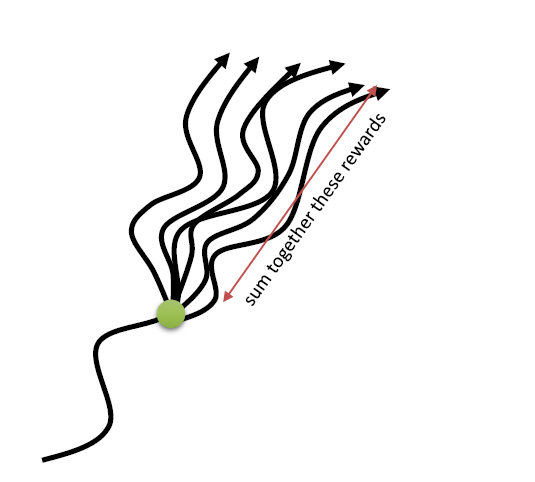
\includegraphics[width=\linewidth]{reward-to-go}
\label{fig:reward-to-go}
\end{marginfigure}
If we know the true "reward to go" $Q(\s_{i,t}, \act_{i,t})$ and replace $\hat{Q}_{i,t}$ with it, we will obtain a better estimation of policy gradient with lower variance which is essential to better convergence.
\begin{equation}
\label{eq:3}
\nabla _\theta J(\theta)  \approx \frac{1}{N} \sum_{i=1} ^ {N} \bigg[\sum_{t=1}^T \nabla_\theta \log \pi_\theta(\act_{i,t}| \s_{i,t})
  Q(\s_{i,t}, \act_{i,t}) \bigg]
\end{equation}
We can also add baseline to the reward estimation:
\begin{equation}
\label{eq:4}
\nabla _\theta J(\theta)  \approx \frac{1}{N} \sum_{i=1} ^ {N} \sum_{t=1}^T \nabla_\theta \log \pi_\theta(\act_{i,t}| \s_{i,t})
  (Q(\s_{i,t}, \act_{i,t}) - b_t)
\end{equation}
We usually choose the average reward as the baseline, so $b_t$ should average over $Q(\s_{i,t}, \act_{i,t})$:
\begin{equation}
\label{eq:5}
b_t = \frac{1}{N} \sum_i Q(\s_{i,t}, \act_{i,t})
\end{equation}
Besides, the expectation of Q-function over policy is the value function:
\begin{equation}
\label{eq:6}
V^\pi (\s_t) = E_{\act_t \sim \pi(\act_t | \s_t)} Q^\pi (\s_t, \act_t)
\end{equation}
We denote that:
\begin{equation}
\label{eq:7}
A^\pi (\s_t, \act_t) = Q^\pi (\s_t, \act_t) - V^\pi(\s_t)
\end{equation}
Where $A^\pi (\s_t, \act_t)$ is referred as \emph{Advantage} which represent how much better $\act_t$ is than the average actions.
Since $b_t$ average over samples drawn from policy distribution $\pi_\theta$, we can substitute $b_t$ with $V(\s_t)$ and the policy gradient should be:
\begin{align}
\label{eq:8}
\nabla _\theta J(\theta)   & \approx \frac{1}{N} \sum_{i=1} ^ {N} \sum_{t=1}^T \nabla_\theta \log \pi_\theta(\act_{i,t}| \s_{i,t})
  (Q(\s_{i,t}, \act_{i,t}) - V(\s_{i, t})) \notag \\
  & = \frac{1}{N} \sum_{i=1} ^ {N} \sum_{t=1}^T \nabla_\theta \log \pi_\theta(\act_{i,t}| \s_{i,t})
  A^\pi(\s_{i,t}, \act_{i,t})
\end{align}
Then the problem is how we  achieve a better estimation of the \emph{Advantage}.
\begin{marginfigure}
    \caption{Diagram of actor-critic. Comparing to REINFORCE algorithm, we fit $Q^\pi$ or $V^\pi$ in model fitting phrase instead of summing over the future rewards.}
    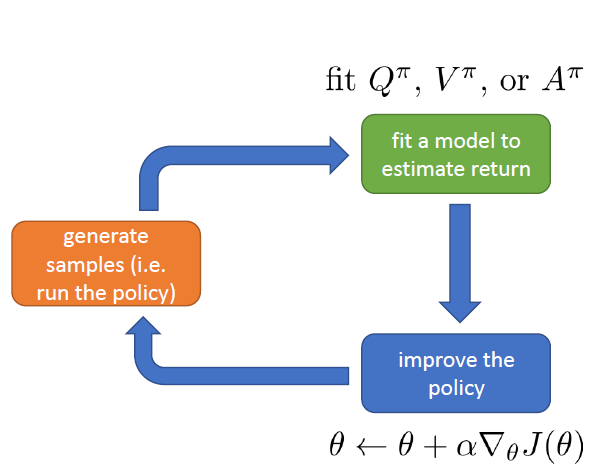
\includegraphics[width=\linewidth]{diagram}
    \label{fig:diagram}
\end{marginfigure}

Intuitively, if we need to compute something complicated, we can use neural network to estimate it. But should we directly estimate the \emph{Advantage}?
From equation \ref{eq:7}, we learned that \emph{Advantage} depends on state and action, and with more inputs, we need more parameters which results in higher variance. Can we estimate \emph{Advantage} with just state or action? To do that, we can take advantage of the relationship between Q-function and
value-function. Firstly, we rewrite $Q^\pi(\s_t, \act_t)$ as sum of the reward at time-step $t$ and expectation of future rewards.
\begin{align}
\label{eq:9}
Q^\pi(\s_t, \act_t) & = r(\s_t, \act_t) + \sum_{t'=t+1}^{T} E_{\pi_\theta} [ r(\s_{t'}, \act_{t'}) | \s_t, \act_t] \notag \\
& = r(\s_t, \act_t) + E_{\s_{t+1} \sim p(\s_{t+1} | \s_t, \act_t)} [ V^\pi (\s_{t+1})]
\end{align}

Besides, the expectation of future rewards is also the expectation of value function at the next time-step $t+1$ which is distributed according to the dynamics of the environment. Then we approximate the expectation with the value function at a specific state $\s_{t+1}$. Obviously, the approximation is not perfect, but from the perspective illustrated in figure \ref{fig:reward-to-go}, we take the first step and estimate the next step with value function which is good enough.
\begin{equation}
\label{eq:10}
Q^\pi(\s_t, \act_t) \approx r(\s_t, \act_t) +  V^\pi (\s_{t+1})
\end{equation}

Moreover, we can estimate \emph{Advantage} with only state.
\begin{equation}
\label{eq:11}
A^\pi(\s_t, \act_t) \approx r(\s_t, \act_t) +  V^\pi (\s_{t+1}) - V^\pi (\s_{t})
\end{equation}

Then we just fit value function $\hat{V} ^\pi _\phi (\s)$ with neural network (parameters denoted as $\phi$) in model-fitting phrase. And the objective is just the expectation of value function of the first state $\s_1$.
\begin{equation}
\label{eq:12}
J(\theta) = E_{\s_1 \sim p(\s_1)} [ V^\pi(\s_1)]
\end{equation}

\subsection{Evaluate with MC}
If we need to fit $\hat{V} ^\pi _\phi (\s)$, what the training example should be? We know the input is $\s_t$, but what the target should be? \ie what's the ground truth of value function? Usually, we use Monte Carlo policy evaluation:
\begin{equation}
\label{eq:13}
V^\pi(\s_t) \approx \frac{1}{N} \sum_{i=1} ^ N \sum_{t'=t}^T r(\s_{t'}, \act_{t'})
\end{equation}

Where we sample trajectories from the state $\s_t$ and average the "reward to go". However, it requires us to reset the simulator to the state $\s_t$ which is impractical. Then what about just the "reward to go" of current trajectory? Since we use neural network as the approximator, it will average the results of value functions with states quiet similar to each other (figure \ref{fig:fit}).

\begin{marginfigure}
\caption{The same function should fit multiple samples, and since the two states are close to each other, the estimated value functions are also close.}
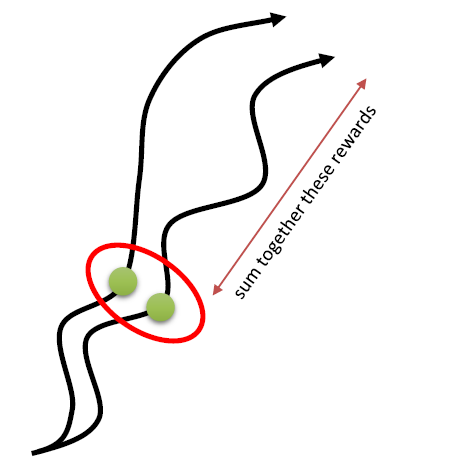
\includegraphics[width=\linewidth]{fit}
\label{fig:fit}
\end{marginfigure}

We denote the target of trajectory $i$ at time-step $t$ as $y_{i,t}$:

\begin{equation}
\label{eq:14}
y_{i,t} = \sum_{t'=t} ^ T r(\s_{i,t'}, \act_{i, t'})
\end{equation}

Then the training data is $\Big\{\Big(\s_{i,t}, \sum_{t'=t} ^ T r(\s_{i,t'}, \act_{i, t'}) \Big) \Big\}$. We construct the learning process as supervised regression where the lost function is the squared distance:

\begin{equation}
\label{eq:15}
\mathcal{L}(\phi) = \frac{1}{2} \sum_i \Big|\Big|\hat{V} ^\pi _\phi (\s_i) - y_i \Big|\Big| ^ 2
\end{equation}

\subsection{Bootstrap mode}

From the perspective of ideal target $y_{i,t}$ (\ie the true value function), can we fit a more accurate $\hat{V}_\phi$?

\begin{align}
\label{eq:16}
y_{i,t} & = \sum_{t'=t} ^ T E_{\pi_\theta} [r(\s_{t'}, \act_{t'}) | \s_{i,t}] \notag \\
& \approx r(\s_{i,t}, \act_{i,t}) +\sum_{t'=t} ^ T E_{\pi_\theta} [r(\s_{t'}, \act_{t'}) | \s_{i,t + 1}] \notag \\
& \approx r(\s_{i,t}, \act_{i,t}) + V^\pi (\s_{i, t+1})
\end{align}

Where we applied the same trick as equation \ref{eq:9}, \ref{eq:10}. The value function could be approximated by the reward of the current time-step plus the value function of the next time-step under the assumption that we took a deterministic action $\act_t$. Then we apply the "bootstrap" trick where we plug in the neural network estimator $\hat{V}_\phi$.

\begin{equation}
\label{eq:17}
y_{i,t} \approx
r(\s_{i,t}, \act_{i,t}) + \hat{V}^\pi _ \phi (\s_{i, t+1})
\end{equation}

The intuition is that if the $\hat{V}_\phi$ is better than cumulative rewards, then use it the estimate the target will "bootstrap" the performance. After
that, the training date should be $\Big\{\Big(\s_{i,t}, r(\s_{i,t}, \act_{i,t}) + \hat{V}^\pi _ \phi (\s_{i, t+1}) \Big) \Big\}$ and we use the same loss function as equation \ref{eq:15}.

In practice, we always initialize the neural network such that the output is small for the sake of stability, \eg making the weights of the last linear layer to be small. Then for the first step, the output of $\hat{V}_\phi$ should look like $r(\s_0, \act_0)$. And the target for the second iteration should be $y_1 = r(\s_0, \act_0) + \hat{V}_\phi(\s_1)$ and $\hat{V}_\phi(\s_1)$ is something look like a reward. Iteratively, it will learn the value function over trajectories after many steps of iterations.

\section{Actor-critic Algorithm}


\subsection{Discount Factors}
However, there is a problem that if $T$ (episode length) is infinite, $\hat{V}_\phi ^ \pi$ can get infinitely large in the case where we want infinite or
approximate infinite episodes \eg training Humanoid robot to run . Hence, we introduce the \emph{discount factor} to address the issue. Suppose that someone grant you a fortune but he will give it to 10 years after, then you may consider to wait cause 10 years is not far away. But if he change it to 100 years after, you may care less cause your descendents can benefit from it. What about 1000 years? The number of years strongly affects the value of the fortune to you. Usually, we prefer the reward which is more reachable \ie better to get rewards sooner than later.
By doing that, we introduce a number $\gamma$ in front of value:
\begin{equation}
\label{eq:18}
y_{i,t} \approx
r(\s_{i,t}, \act_{i,t}) + \gamma \hat{V}^\pi _ \phi (\s_{i, t+1})
\end{equation}

Where $\gamma \in [0, 1]$, and usually $0.99$ works pretty well. From the perspective of MDP, $\gamma$ changes the transition probability:

\begin{equation}
\label{eq:19}
\hat{p}(\s' | \s, \act) = \gamma p(\s' | \s, \act)
\end{equation}

Is $\gamma$ a parameter of the \emph{critic}? Actually, $\gamma$ is just the property of the MDP and highly depends on the problem setting.

How can we plug $\gamma$ in policy gradient (equation \ref{eq:1})? There are two options:

\textbf{Option 1:}

After we apply the property of causality as equation \ref{eq:1}, we can plug $\gamma$ directory in front of the reward.

\begin{equation}
\label{eq:20}
\nabla _\theta J(\theta) \approx \frac{1}{N} \sum_{i=1} ^ {N} \bigg[\sum_{t=1}^T \nabla_\theta \log \pi_\theta(\act_{i,t}| \s_{i,t})
\Big( \sum_{t'=t}^T \gamma ^ {t' - t} r(\s_{i, t'}, \act_{i, t'}) \Big) \bigg]
\end{equation}

\textbf{Option 2:}

Another option is to plug in $\gamma$ before temporal decomposed policy gradient.

\begin{align}
\label{eq:21}
\nabla _\theta J(\theta)
& \approx \frac{1}{N} \sum_{i=1} ^ {N} \bigg[\Big(\sum_{t=1}^T \nabla_\theta \log \pi_\theta(\act_{i,t} | \s_{i,t}) \Big)
\Big( \sum_{t=1}^T \gamma^{t - 1} r(\s_{i,t}, \act_{i,t}) \Big) \bigg] \notag \\
& = \frac{1}{N} \sum_{i=1} ^ {N} \sum_{t=1}^T \nabla_\theta \log \pi_\theta(\act_{i,t} | \s_{i,t})
\Big( \sum_{t'=1}^T \gamma^{t' - 1} r(\s_{i,t'}, \act_{i,t'}) \Big)  \notag \\
& = \frac{1}{N} \sum_{i=1} ^ {N} \sum_{t=1}^T \gamma ^ {t - 1} \nabla_\theta \log \pi_\theta(\act_{i,t} | \s_{i,t})
\Big( \sum_{t'=t}^T \gamma^{t' - t} r(\s_{i,t'}, \act_{i,t'}) \Big)
\end{align}

Obviously, the two options are not the same. Option 2 discounts the gradient from step 1 \ie later steps matter less, which is quiet reasonable.
However, we usually use option 1 in practice which is approximating the average reward as in the infinite horizon tasks, and Philip Thomas et al.
discussed it in the paper "Bias in natural actor-critic algorithms" (\href{http://proceedings.mlr.press/v32/thomas14.html}{link}).

\subsection{Batch Actor-critic algorithm}

With policy evaluation with estimated value function, we derived the batch actor-critic algorithm by plugging value function estimation to REINFORCE algorithm:

\begin{algorithm}
  \caption{Batch Actor-critic Algorithm}
    \label{algo:batch-ac}
    \begin{algorithmic}[1]
    % \REQUIRE some words.  % this command shows "Input"
    % \ENSURE
    \WHILE {\emph{Not converged}}
    \STATE sample $\{\s_i, \act_i \} $ from $\pi_\theta(\act | \s)$ by running the policy. \\
    \STATE Fit $\hat{V}_\phi ^ \pi (\s)$ to sampled reward sums. \\
    \STATE Evaluate $\hat{A}^\pi(\s_i, \act_i) \approx r(\s_i, \act_i) + \gamma \hat{V}^\pi_\phi (\s'_{i}) - \hat{V}^\pi_\phi(\s_{i})$
    \STATE $\nabla _\theta J(\theta) \approx 1/N \sum_{i=1} ^ {N} \nabla_\theta \log \pi_\theta(\act_i| \s_i) \hat{A}^\pi(\s_i, \act_i)$ \\
    \STATE $ \theta \leftarrow \theta + \alpha \nabla _\theta J(\theta)$ \\
    \ENDWHILE
    \RETURN trained $\pi_\theta$  % this command shows "Output"
  \end{algorithmic}
\end{algorithm}

We often refer $\hat{V}_\phi ^ \pi (\s)$ as the \emph{critic}. During training, we generate batch of trajectories. And for the $\hat{V}_\phi ^ \pi (\s)$ fitting step, one can choose to update $\hat{V}_\phi ^ \pi (\s)$ for many iterations, or just train one-time for speeding up. For the fitting method, bootstrap is more popular than Monte Carlo evaluation.

\subsection{Online Actor-critic Algorithm}

We can also derive the on-line version of actor-critic algorithm, where after each time we take a step, we estimate the value function and update the policy.

\begin{algorithm}
  \caption{Online Actor-critic Algorithm}
    \label{algo:online-ac}
    \begin{algorithmic}[1]
    % \REQUIRE some words.  % this command shows "Input"
    % \ENSURE
    \WHILE {\emph{Not converged}}
    \STATE Take action $\act \sim \pi_\theta(\act| \s)$, get $(\s, \act, \s', r)$. \\
    \STATE Update $\hat{V}_\phi ^ \pi$ with $r + \gamma \hat{V}_\phi ^ \pi (\s') $. \\
    \STATE Evaluate $\hat{A}^\pi(\s, \act) \approx r(\s, \act) + \gamma \hat{V}^\pi_\phi (\s') - \hat{V}^\pi_\phi(\s)$ \\
    \STATE $\nabla _\theta J(\theta) \approx \nabla_\theta \log \pi_\theta(\act| \s) \hat{A}^\pi(\s, \act)$ \\
    \STATE $ \theta \leftarrow \theta + \alpha \nabla _\theta J(\theta)$ \\
    \ENDWHILE
    \RETURN trained $\pi_\theta$  % this command shows "Output"
  \end{algorithmic}
\end{algorithm}

\subsection{Architecture Design}
\begin{marginfigure}
\caption{Two network design}
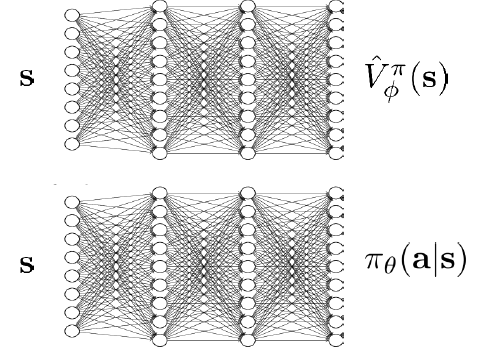
\includegraphics[width=\linewidth]{two-net}
\label{fig:two-net}
\end{marginfigure}

\begin{marginfigure}
\caption{Shared network design}
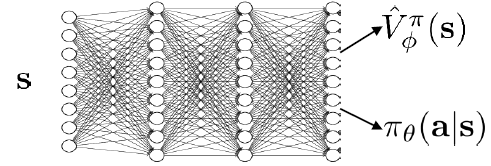
\includegraphics[width=\linewidth]{one-net}
\label{fig:one-net}
\end{marginfigure}

We need to estimate \emph{critic} $\hat{V}_\phi ^ \pi (\s)$ and the policy $\pi_\theta(\act | \s)$. Naturally, we can achieve the estimation with two explicit networks (figure \ref{fig:two-net}), it's simple and stable for training without heavy tuning, but there is no shared features between actor and
critic. Another option is taking advantage of the mutual features as in common CV tasks where the basic features like line, circle is mutual for different task. With the shared network design (figure \ref{fig:one-net}), we use two heads as the prediction of actor and critic which is more efficient \thanks{AlphaGo Zero used the shared network to train the actor and critic}. The shortage is that the shared network is tougher to train cause we push different kinds of gradients to the backbone.

\subsection{Parallelism}

We learned the the two main problems of policy gradient are high variance and slow convergence, and we are trying to address the high variance issue
with causality and baseline trick. However, for the one-line actor-critic algorithm where we estimate $\hat{V}_\phi ^ \pi (\s)$ and policy
$\pi_\theta(\act | \s)$ with data of a single step, it contributes to higher the variance. One way to deal with that is working with a batch \ie increasing the samples to reduce variance. A practical way to do it is using parallel workers.

\textbf{Synchronized parallel actor-critic}:

Suppose that we have four workers (figure \ref{fig:sync}) and each worker works independently. During training, each worker takes a step and collects data
$(\s, \act, \s', r)$. When all the workers finishing collecting data, the main worker collects the four samples and updates the policy. In this way, we have
four times examples. Obviously, the more worker we have, the lower variance and faster convergence it will be. However parallelism is not trivial in some
cases, and we need to make the trade-off.

\begin{marginfigure}
\caption{Synchronized parallel actor-critic}
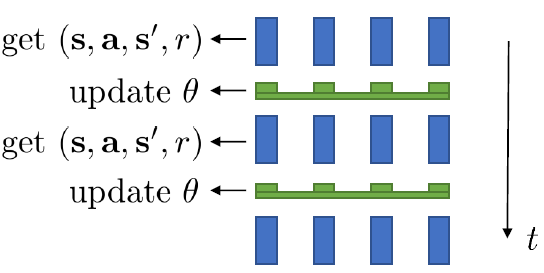
\includegraphics[width=\linewidth]{sync}
\label{fig:sync}
\end{marginfigure}

\textbf{Asynchronous parallel actor-critic:}

The synchronized version could be comparably slow, we have to wait until all workers has finished data collecting to update the policy. Another more
advanced scheme is \emph{asynchronous parallelism} (figure \ref{fig:async}) where we have multiple workers and a parameter server which is responsible for
storing and updating parameter $\theta$. Once any worker has finished collecting data, it sends the estimated gradient to parameter server and updating policy immediately. At the same time, the other worker may still works with old parameters.

\begin{marginfigure}
\caption{Asynchronous parallel actor-critic}
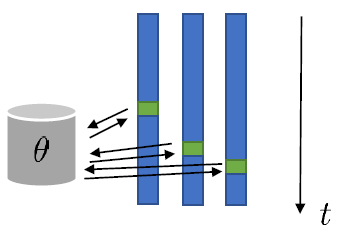
\includegraphics[width=\linewidth]{async}
\label{fig:async}
\end{marginfigure}

\subsection{State-dependent Baselines}

The REINFORCE algorithm (equation \ref{eq:20}) is unbiased estimation w.r.t policy gradient, since adding the constant baselines has no impact on gradients.
But it has high variance due to single-sample estimation of "reward to go". The actor-critic algorithm (\ref{algo:batch-ac}) has lower variance due to critic. However, it's not biased as the neural network approximation is not perfect. One clever way to combining the advantage of the algorithms is using
$\hat{V}_\phi ^ \pi (\s)$ as the baseline and keeping the naive "reward to go" estimation.
\begin{equation}
\label{eq:22}
\nabla _\theta J(\theta) \approx \frac{1}{N} \sum_{i=1} ^ {N} \bigg[\sum_{t=1}^T \nabla_\theta \log \pi_\theta(\act_{i,t}| \s_{i,t})
\Big( \sum_{t'=t}^T \gamma ^ {t' - t} r(\s_{i, t'}, \act_{i, t'}) - \hat{V}_\phi ^ \pi (\s_{i,t}) \Big) \bigg]
\end{equation}

Where the baselines is $\hat{V}_\phi ^ \pi (\s)$ which is only state-dependent, and during differentiating w.r.t $\theta$, it could be seen as a
\emph{constant}, just like the average baseline $b$. And the result enjoys the benefits of unbiased estimation and lower variance compared to REINFORCE
algorithm.

\subsection{Action-dependent Baselines}
Adding only state-dependent baselines, we will have an unbiased and higher variance estimation of \emph{advantage}. But if we also incorporate action into the baseline, the difference between "reward to go" and baselines gets lower, even goes to zero in expectation if critic is correct. \thanks{If the policy is deterministic, it will probably go to zero.}
\begin{equation}
\label{eq:23}
\hat{A}^\pi (\s_t, \act_t) = \sum_{t'=t}^T \gamma ^ {t' - t} r(\s_{ t'}, \act_{t'}) - \hat{Q}_\phi ^ \pi (\s_{t}, \act_t)
\end{equation}
However, the resulting policy gradient is biased as the baselines $\hat{Q}_\phi ^ \pi (\s_{t}, \act_t)$ depends on action. But we can manage to make it unbiased with adding a extra term\thanks{More about variance reduction later}.
\begin{align}
\label{eq:24}
\nabla _\theta J(\theta) \approx & \frac{1}{N} \sum_{i=1} ^ {N} \bigg[\sum_{t=1}^T \nabla_\theta \log \pi_\theta(\act_{i,t}| \s_{i,t})
\Big( \sum_{t'=t}^T \gamma ^ {t' - t} r(\s_{i, t'}, \act_{i, t'}) - \hat{Q}_\phi ^ \pi (\s_{i,t}) \Big) \bigg] \notag \\
& + \frac{1}{N} \sum_{i=1} ^ {N} \sum_{t=1}^T \nabla_\theta E_{\act \sim \pi_\theta (\act_t | s_{i,t})} \Big[\hat{Q}_\phi ^ \pi (\s_{i,t}, \act_t) \Big]
\end{align}
Following the proof of constant baselines is unbiased (lecture 3), we could obtain that:
\begin{equation}
\label{eq:25}
\frac{1}{N} \sum_{i=1} ^ {N} \sum_{t=1}^T \nabla_\theta \log \pi_\theta(\act_{i,t}| \s_{i,t})
\hat{Q}_\phi ^ \pi (\s_{i,t}) =
\frac{1}{N} \sum_{i=1} ^ {N} \sum_{t=1}^T \nabla_\theta E_{\act \sim \pi_\theta (\act_t | s_{i,t})} \Big[\hat{Q}_\phi ^ \pi (\s_{i,t}, \act_t) \Big]
\end{equation}
Then with equation \ref{eq:24}, we use the action-dependent baselines provided the second term can be evaluated \eg the case where
 $\hat{Q}_\phi ^ \pi$ is quadratic and the policy $\pi_\theta$ is distributed according to Gaussian distribution. It's referred as \emph{control variates}.

\subsection{Generalized Advantage Estimation}

The actor-critic (algorithm \ref{algo:batch-ac}) has lower variance but higher bias due to the value function estimation is not accurate, and the
REINFORCE with state-dependent baselines (equation \ref{eq:22}) has no bias but higher variance due to single-sampled estimation of "reward to go".

\begin{equation}
\label{eq:26}
\hat{A}_C^\pi (\s_t, \act_t) = r(\s_t, \act_t) + \gamma \hat{V} ^\pi_\phi(\s_{t+1} - \hat{V}^\pi_\phi(\s_t))
\end{equation}

\begin{equation}
\label{eq:27}
\hat{A}_{MC}^\pi (\s_t, \act_t) = \sum_{t'=t}^\infty r(\s_{t'}, \act_{t'}) - \hat{V}^\pi_\phi(\s_t))
\end{equation}

So can we combine these ideas to control the bias-variance trade-off?

The intuition is that starting from a state, the further to the future, the higher the variance will be. So at the closer region to the starting point, the estimation has low variance. Then we can try to draw a "line" after several steps to stopping estimating with single sample and plug in the value function to estimate for the future.

\begin{marginfigure}
\centering
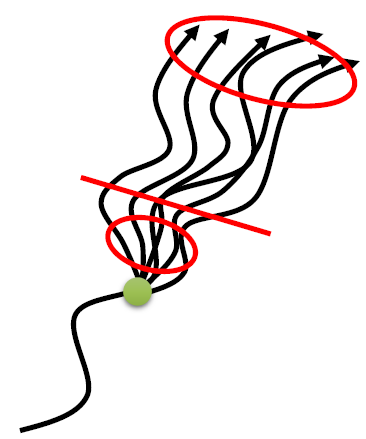
\includegraphics[width=\linewidth]{n-step}
\caption{Illustration of bias-variance trade-off with a cutting line not far from the current state}
\label{fig:n-step}
\end{marginfigure}

Another way to look at it is that, the difference between equation \ref{eq:26} and \ref{eq:27} is, actor-critic is the reward of \emph{one-step} plus discounted future value as the "reward to go", and REINFORCE with value critic is cumulative rewards of \emph{all time-steps} as the "reward to go". One straightforward way to control the trade-off is changing the number of steps (from 1 to $T$) to sum and plugging in discounted value for the future. Sometimes, it's referred as \emph{n-step returns}.

\begin{equation}
\label{eq:28}
\hat{A}_n^\pi (\s_t, \act_t) =\sum_{t'=t} ^ {t+n} r(\s_{t'}, \act_{t'}) + \gamma^{n} \hat{V} ^\pi_\phi(\s_{t+n} - \hat{V}^\pi_\phi(\s_t))
\end{equation}

In practice, choosing $n > 1$ often works better. \thanks{During early stages of training, choose $n = 4$ or $5$ contributes faster learning. }

Going further from the idea, what about choosing different $n$ and finding a way to blend all? It leads the \emph{generalized advantage estimation} where
we take n from current time-step to the end $T$ and blend all with wighted combination of n-step returns.

\begin{equation}
\label{eq:29}
\hat{A}^\pi _{GAE}(\s_t, \act_t) = \sum_{n=1}^T w_n \hat{A}_n^\pi (\s_t, \act_t)
\end{equation}

With the intuition of the closer to current time step, lower variance it is, we choose the weights proportional to exponent of parameter $\lambda$:

\begin{equation}
\label{eq:30}
w_n = {\lambda ^ {n -1}}{(1 - \lambda)}
\end{equation}

With some derivation \thanks{Refer \href{https://arxiv.org/pdf/1506.02438.pdf}{\underline{paper}} of Schulman et al. for details of derivation.},
the GAE is:

\[
\hat{A}^\pi _{GAE}(\s_t, \act_t) = \sum_{n=1}^T (\gamma \lambda) ^{t' - t} \delta_{t'}
\]

where

\[
\delta_{t'} = r(\s_{t'}, \act_{t'}) + \gamma \hat{V} ^\pi_\phi (\s_{t' + 1} - \hat{V} ^\pi_\phi (\s_{t'} )
\]

When $\lambda = 0$, it reduces to equation \ref{eq:26} and $\lambda = 1$, it is the same as equation \ref{eq:27}. Then we can choose
$\lambda \in [0, 1]$ to control the bias-variance trade-off.

\section{Suggested Readings}

\begin{itemize}
   \item [\textbf{Classic Papers}]
   \item Sutton et al. Policy gradient methods for reinforcement learning with function approximation: actor-critic algorithms with value function approximation.
   \href{https://papers.nips.cc/paper/1713-policy-gradient-methods-for-reinforcement-learning-with-function-approximation.pdf}{\underline{link}}.

   \item [\textbf{Recent Deep RL}]
   \item Mnih et al. Asynchronous methods for deep reinforcement learning: A3C with parallel online actor-critic.
   \href{https://arxiv.org/abs/1602.01783}{\underline{link}}.
   \item Schulman et al. High-dimensional continuous control using generalized advantage estimation: batch-mode actor-critic with blended Monte Carlo
   and function approximator returns.
   \href{https://arxiv.org/pdf/1506.02438.pdf}{\underline{link}}.
   \item Gu et al. Q-prob: sample efficient policy-gradient with an off-policy critic: policy gradient with Q-function control variate.
   \href{https://arxiv.org/abs/1611.02247}{\underline{link}}.


\end{itemize}


\end{document}
